% !TEX program = lualatex 

\documentclass[9pt]{beamer}

\usetheme{metropolis}
\usepackage{bookmark}
\usepackage{xcolor-solarized}

\setbeamercolor{normal text}{%
  fg=solarized-base02,
  bg=solarized-base3!20!white
}
\setbeamercolor{alerted text}{%
  fg=solarized-red
}
\setbeamercolor{example text}{%
  fg=solarized-green
}
\setbeamercolor{frametitle}{%
    fg=solarized-blue!70!black,
    bg=solarized-base2
}

\setbeamerfont{title}{series=\bfseries,parent=structure}
\setbeamerfont{frametitle}{series=\bfseries,parent=structure}
\renewcommand{\footnotesize}{\scriptsize}

\usecolortheme{orchid}

\usepackage{hott}
\usepackage{mathtools}
\usepackage{macros}
\usepackage[final]{microtype}

\usepackage{worldflags}
\usepackage{mathpartir}
\usepackage{stmaryrd}
\usepackage{lipsum}
\usepackage{adjustbox}
\usepackage{amsmath}
\usepackage{amssymb}
\usepackage{geometry}
\usepackage{mathrsfs}
\usepackage{braket}
\usepackage{quiver}
\usepackage{mathtools}
\usepackage{commath}
\usepackage{xparse}
\usepackage{array}
\usepackage{subcaption} %side by side diagrams
\usepackage{floatrow}
\usepackage{tikz}
\usepackage{tikz-cd}
\usetikzlibrary{babel}% added

% bibliography
\usepackage[style=authortitle,backend=biber]{biblatex}
\addbibresource{../symmetries.bib}

% fancy boxes
\usepackage[most]{tcolorbox}

\newtcolorbox{qblock}[1][Question]{
  colback=white,
  colframe=solarized-orange,
  colbacktitle=white!90!structure.fg,
  coltitle=black,
  fonttitle=\itshape,
  title={#1},
  enhanced,
  attach boxed title to top left={yshift=-0.1cm, xshift=0.5em}
}
\newtcolorbox{dblock}[1][Definition]{
  colback=white,
  colframe=solarized-violet,
  colbacktitle=white!90!structure.fg,
  coltitle=black,
  fonttitle=\itshape,
  title={#1},
  enhanced,
  attach boxed title to top left={yshift=-0.1cm, xshift=0.5em}
}

\newtcolorbox{pblock}[1][Proposition]{
  colback=white,
  colframe=solarized-blue,
  colbacktitle=white!90!structure.fg,
  coltitle=black,
  fonttitle=\itshape,
  title={#1},
  enhanced,
  attach boxed title to top left={yshift=-0.1cm, xshift=0.5em}
}

\newtcolorbox{tblock}[1][Theorem]{
  colback=white,
  colframe=solarized-green,
  colbacktitle=white!90!structure.fg,
  coltitle=black,
  fonttitle=\itshape,
  title={#1},
  enhanced,
  attach boxed title to top left={yshift=-0.1cm, xshift=0.5em}
}

\usepackage{tikz}
\usetikzlibrary{cd}
\usetikzlibrary{fit}

\usepackage{fontspec}
\setmonofont{Iosevka}[
    Path=./Iosevka/,
    Extension = .ttf,
    UprightFont=*-Regular,
    BoldFont=*-Bold,
    ItalicFont=*-Italic,
    BoldItalicFont=*-BoldItalic
]

% sort
\newcommand{\issortedany}{\term{in-image}}
\newcommand{\issorted}{\issortedany_s}
\newcommand{\isheadleast}{\term{image-respects-pair}}
\newcommand{\istailsort}{\term{image-can-induct}}
\newcommand{\setord}{\term{Ord}}
\newcommand{\Ord}{\term{Ord}}
\newcommand{\setmtol}{\term{M2L}}
\newcommand{\setsort}{\term{Sort}}
\newcommand{\Sort}{\term{Sort}}
\newcommand{\otof}{\term{o2f}}
% constructions
\newcommand{\List}{\term{List}}
\newcommand{\Array}{\term{Array}}
\newcommand{\PList}{\term{PList}}
\newcommand{\SList}{\term{SList}}
\newcommand{\Bag}{\term{Bag}}
\newcommand{\Perm}{\term{Perm}}

%Information to be included in the title page:
\title{On commutativity, total orders, and sorting}
\author[shortname]{
  Wind Wong \inst{1}
  \and Vikraman Choudhury \inst{2}
  \and Simon J. Gay \inst{1}
}
\institute[shortinst]{\inst{1} University of Glasgow \and %
                      \inst{2} Universit\`{a} di Bologna and OLAS Team, INRIA}
\date{February 14, 2024}

\AtBeginSection[]{%
  \begin{frame}<beamer>
    \frametitle{Outline}
    \tableofcontents[sectionstyle=show/shaded,subsectionstyle=hide/show/hide]
  \end{frame}
}

\begin{document}

\frame{\titlepage}

\section{Introduction}

\begin{frame}
  \frametitle{Introduction}
  In this talk, we study constructions of
  \alert{free monoids} and \alert{free commutative monoids}.

  We created a framework for \alert{universal algebra} to study these constructions!

  We apply this framework to study the relationship
  between \alert{sorting} and \alert{total orders}:

  \begin{center}
      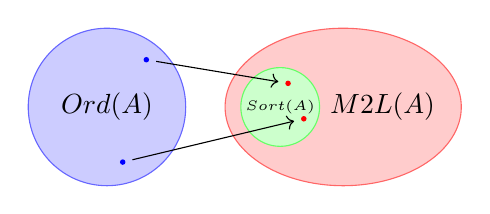
\begin{tikzpicture}
          % draw the sets
          \filldraw[fill=blue!20, draw=blue!60] (-1.5,0) circle (1cm);
          \filldraw[fill=red!20, draw=red!60] (1.5,0) ellipse (1.5cm and 1cm);
          \filldraw[fill=green!20, draw=green!60] (0.7,0) circle (0.5cm);
      
          % the texts
          \node at (-1.5,0) {$\Ord(A)$};
          \node at (0.7, 0) {\tiny$\Sort(A)$};
          \node at (2,0) {$\setmtol(A)$};
  
      
          % the points in the sets (here I just create nodes to use them later on to position
          % the circles and the arrows
          \node (x1) at (-1,0.6) {};
          \node (x2) at (-1.3,-0.7) {};
          \node (y1) at (0.8,0.3) {};
          \node (y2) at (1,-0.15) {};
      
          % position the elements in the sets (at the nodes we just created)
          \fill[blue] (x1) circle (1pt);
          \fill[blue] (x2) circle (1pt);
          \fill[red] (y1) circle (1pt);
          \fill[red] (y2) circle (1pt);
      
          % draw the arrows
          \draw[->] (x1) -- (y1);
          \draw[->] (x2) -- (y2);
      \end{tikzpicture}
  \end{center}

  Sorting functions are a subset of functions $\term{UnorderedList(A)} \to \List(A)$.
  Can we construct total orders from sorting functions?

\end{frame}

\section{Background: Universal Algebra}

\begin{frame}[fragile]{Universal Algebra}
\frametitle{Universal Algebra}

A \alert{signature} $\sigma$ is:
\begin{itemize}
    \item a set of \alert{function symbols} $op : \mathsf{hSet}$
    \item an \alert{arity function} $ar : op \rightarrow \mathsf{hSet}$
\end{itemize}

This gives a signature endofunctor $F_{\sigma}(X) := \sum_{f : op} X^{ar(f)}$

A $\sigma$-structure is a $F_{\sigma}$-algebra:
\begin{itemize}
    \item a \alert{carrier set} $X : hSet$
    \item an \alert{interpretation function}: $\alpha_X\colon\Sig(X) \to X$
\end{itemize}

A $\sigma$-algebra homomorphism $h: X \rightarrow Y$ is a function such that:
% https://q.uiver.app/#q=WzAsNCxbMCwwLCJGX3tcXHNpZ21hfShYKSJdLFsxLDAsIlgiXSxbMCwxLCJGX3tcXHNpZ21hfShZKSJdLFsxLDEsIlkiXSxbMCwxLCJcXGFscGhhX1giXSxbMCwyLCJGX3tcXHNpZ21hfShoKSIsMl0sWzIsMywiXFxhbHBoYV9ZIiwyXSxbMSwzLCJoIl1d
\[\begin{tikzcd}[ampersand replacement=\&,cramped]
	{F_{\sigma}(X)} \& X \\
	{F_{\sigma}(Y)} \& Y
	\arrow["{\alpha_X}", from=1-1, to=1-2]
	\arrow["{F_{\sigma}(h)}"', from=1-1, to=2-1]
	\arrow["{\alpha_Y}"', from=2-1, to=2-2]
	\arrow["h", from=1-2, to=2-2]
\end{tikzcd}\]

$F_{\sigma}$-algebras and their morphisms form a category $\sigma$-Alg.

Example: $\mathbb{N}$ as a \alert{lawless monoid}:
The signature $\sigma_{\mathsf{Mon}}$ has:
$op : \mathsf{hSet} = \{\munit, \mmult\}$ (or $\Fin[2]$ or $\Bool$),
$ar : \sigma \rightarrow \mathsf{hSet} = \{\munit \mapsto \Void,, \mmult \mapsto \Bool\}$

\end{frame}


\begin{frame}{Free Algebras}
The free $\sigma$-algebra $\mathfrak{F}(X)$ on a carrier set $X$, \alert{if it exists}, produces a \alert{left adjoint} to the forgetful functor $\sigma$-Alg to $\hSet$, given by:
\begin{itemize}
    \item a type constructor $F : \mathsf{hSet} \to \mathsf{hSet}$,
    \item a universal generators map $\eta_X : X \to F(X)$, such that
    \item for any $\sigma$-algebra $\mathfrak{Y}$, post-composition with $\eta_X$ is an equivalence.
    %% \[
    %%     (F(V) \xto{f} \mathfrak{Y}) \quad\mapsto\quad (V \xto{\eta_V} F(X) \xto{f} Y)
    %% \]
    %% is an equivalence.
\end{itemize}

% \begin{dblock}[Universal property of free algebras]
% For any object \( \mathfrak{Y} \) in $\sigma$-Alg, $(\blank) \circ \eta_X$ is an equivalence:
% 
% % https://q.uiver.app/#q=WzAsMyxbMCwwLCJYIl0sWzIsMCwiVShBKSJdLFsyLDIsIlUoQikiXSxbMCwxLCJpIiwwLHsiY29sb3VyIjpbMSwxMDAsNjBdfSxbMSwxMDAsNjAsMV1dLFswLDIsImciLDJdLFsxLDIsIlUoZikiLDAseyJzdHlsZSI6eyJib2R5Ijp7Im5hbWUiOiJkb3R0ZWQifX19XV0=
% \[
% \begin{tikzcd}[ampersand replacement=\&]
% 	\mathfrak{F}(X) \\
% 	\\
% 	\mathfrak{Y}
% 	\arrow["f", dotted, from=1-1, to=3-1]
% \end{tikzcd}
% \mapsto
% \begin{tikzcd}[ampersand replacement=\&]
% 	X \&\& {F(X)} \\
% 	\\
% 	\&\& {Y}
% 	\arrow["\eta_X", color={rgb,255:red,255;green,54;blue,51}, from=1-1, to=1-3]
% 	\arrow["f \comp \eta_X"', from=1-1, to=3-3]
% 	\arrow["{f}", dotted, from=1-3, to=3-3]
% \end{tikzcd}\]
% 
% %% where $U$ is the forgetful functor and $\eta_X : X \rightarrow F(X)$ is the canonical injection.
% 
% The inverse is the extension operation: $\ext{(\blank)}\colon (X \to Y) \to \mathfrak{F}(X) \to \mathfrak{Y}$. $F(X)$ is unique upto (unique) isomorphism.
% \end{dblock}

In type theory, this always exists! 

\end{frame}
\begin{frame}
\frametitle{Free Algebras}
We define the carrier set using an inductive type of trees $Tr_\sigma(V)$, generated by two constructors:
\begin{itemize}
    \item $\text{leaf} : V \rightarrow Tr_\sigma(V)$, and
    \item $\text{node} : F_{\sigma}(Tr_\sigma(V)) \rightarrow Tr_\sigma(V)$.
\end{itemize}

Expanding node: $(f: op) \times (\mathsf{ch}: ar(f) \to Tr_{\sigma}(V)) \to Tr_{\sigma}(V)$.

node is our \alert{algebra map} $\alpha : F_\sigma(Tr_\sigma(V)) \rightarrow Tr_\sigma(V)$.
%% node is our \alert{interpretation function} $\alpha : F_\sigma(Tr_\sigma(V)) \rightarrow Tr_\sigma(V)$


leaf is our \alert{generators map} $\eta : V \rightarrow Tr_\sigma(V)$.

This gives a $\sigma$-algebra $\str{T}(V) = (\tree{V}, \term{node})$.

% By the \alert{universal property}: $(\blank) \comp \eta \colon \sigAlg(\str{T}(V),\str{X}) \xto{\sim} (V \to X)$.

\begin{tblock}
  $\str{T}(V)$ is the free $\sigma$-algebra on $V$.
\end{tblock}

% The inverse to the equivalence: the \alert{extension operation} $\ext{(\blank)}$,
% maps $f\colon V \to X$ to a homomorphism $\ext{f}\colon \str{T}(V) \to \str{X}$.~\footnote{In functional programming (recursion schemes), $\ext{(\blank)}$ is like a \alert{fold}/\alert{catamorphism}.}
\end{frame}

\begin{frame}
\frametitle{Free Algebras}
  $Tr_\sigma(V)$ can be represented by the W-type:
\begin{itemize}
  \item the \alert{shape} $S : \UU$ given by $V + op_\sigma$,
  \item the \alert{family of positions} $P : S \to \UU$ given by
    $\{ inl(v) \mapsto \bot, inr(v) \mapsto ar_\sigma \}$.
\end{itemize}

Trees for $\sigma_{\term{Mon}}$ with the carrier set $\Nat$ would look like:
\begin{center}
\scalebox{0.7}{
% https://q.uiver.app/#q=WzAsNixbMiwyLCIrIl0sWzIsMywiNCJdLFszLDEsIisiXSxbMiwwLCIxIl0sWzQsMCwiMSJdLFswLDAsIjIiXSxbMCwxXSxbMiwwXSxbMywyXSxbNCwyXSxbNSwwXV0=
\begin{tikzcd}[ampersand replacement=\&,cramped]
	2 \&\& 1 \&\& 1 \\
	\&\&\& {+} \\
	\&\& {+} \\
	\&\&
	\arrow[no head, from=3-3, to=4-3]
	\arrow[from=2-4, to=3-3]
	\arrow[from=1-3, to=2-4]
	\arrow[from=1-5, to=2-4]
	\arrow[from=1-1, to=3-3]
\end{tikzcd}
\hspace{2em}
% https://q.uiver.app/#q=WzAsNixbMiwyLCIrIl0sWzIsMCwiMSJdLFs0LDAsIjEiXSxbMCwwLCIyIl0sWzEsMSwiKyJdLFsyLDNdLFszLDRdLFs0LDBdLFsxLDRdLFsyLDBdLFswLDUsIiIsMCx7InN0eWxlIjp7ImhlYWQiOnsibmFtZSI6Im5vbmUifX19XV0=
\begin{tikzcd}[ampersand replacement=\&,cramped]
	2 \&\& 1 \&\& 1 \\
	\& {+} \\
	\&\& {+} \\
	\&\& {}
	\arrow[from=1-1, to=2-2]
	\arrow[from=2-2, to=3-3]
	\arrow[from=1-3, to=2-2]
	\arrow[from=1-5, to=3-3]
	\arrow[no head, from=3-3, to=4-3]
\end{tikzcd}
}
\end{center}

These trees should be equivalent by associativity since they are trees of a monoid...

\end{frame}

\begin{frame}
\frametitle{Universal Algebra}
So far there are no \alert{laws}! How do we add \alert{laws}?

An \alert{equational signature} $\varepsilon$ is given by:
\begin{itemize}
    \item a set of \alert{equation symbols} $eq : \hSet$,
    \item an \alert{arity of free variables} $fv : eq \to \hSet$
\end{itemize}

A system of equations (or \alert{equational theory} $T_{\varepsilon}$) is a pair of trees on the set of free variables:
$l, r : (e : eq) \to Tr_\sigma(fv(e))$

$\mathfrak{X}$ satisfies $T$ ($\mathfrak{X} \entails T$) if for all $e : eq$ and $\rho : fv(e) \to V$,
$\ext{\rho}(l(e)) = \ext{\rho}(r(e))$

Concretely:
\begin{itemize}
    \item $\rho : fv(e) \to V$ assigns free variables in equations to elements of $V$
    \item $\ext{\rho} : Tr_\sigma(fv(e)) \to V$ evaluates a tree given an assignment of free variables
\end{itemize}

Because $\ext{\rho}$ is a \alert{homomorphism}, it must evaluate the tree correctly!

\end{frame}

\begin{frame}
\frametitle{Universal Algebra}
Example: $\mathbb{N}$ is a (lawful) \alert{monoid}.

The equational signature $\sigma_{\mathsf{Mon}}$ has:
\begin{itemize}
    \item the set of \alert{equation symbols} $eq = \{\text{unitl}, \text{unitr}, \text{assocr}\}$
    (or $\Fin[3]$ or $\mathbf{3}$),
    \item the \alert{arity function}
    $fv : eq \rightarrow \mathsf{hSet} = \{\text{unitl} \mapsto \mathbf{1}, \text{unitr} \mapsto \mathbf{1}, \text{assocr} \mapsto \mathbf{3}\}$.
\end{itemize}

To show $(\Nat,0,+) \entails \text{Mon}$:
\begin{align*}
unitl  & : \forall (\rho : \Nat^{\Fin[1]}). \, \rho(0) + 0 \id \rho(0) \\
unitr  & : \forall (\rho : \Nat^{\Fin[1]}). \, 0 + \rho(0) \id \rho(0) \\
assocr & : \forall (\rho : \Nat^{\Fin[3]}). \, (\rho(0) + \rho(1)) + \rho(2) \id \rho(0) + (\rho(1) + \rho(2))
\end{align*} 

The $\sigma$-algebras satisfying a theory $T_{\varepsilon}$ form a subcategory $(\sigma,\varepsilon)$-Alg (or a variety of algebras).
\end{frame}

\begin{frame}
\frametitle{Universal Algebra}
In this talk, we only consider the construction of free objects for the special case of \alert{monoids} and \alert{commutative monoids}.

But can we construct any arbitrary free algebras?

As a quotient of tree:
\begin{itemize}
  \item Need choice to handle \alert{infinitary} operations!
  \item We can only construct free algebras for \alert{finitary} operations.  
\end{itemize} 

As a HIT:
\begin{itemize}
  \item We \alert{don't} need choice for \alert{infinitary} operations!
  \item But Cubical Agda complains about positivity.
\end{itemize}

We didn't investigate further, but it should be possible to construct arbitrary free algebras
in Cubical Agda.

\end{frame}

\section{Free (commutative) monoids}

\begin{frame}[fragile]{Constructions of free (commutative) monoids}
    % There are various well-known constructions of free monoids~\footcite{dubucFreeMonoids1974,kellyUnifiedTreatmentTransfinite1980}.
    It's well known that Lists are free monoids:

%     \begin{dblock}[Cons Lists]
%         \begin{code}
% data List (A : UU) : UU where
%   nil : List A
%   _cons_ : A -> List A -> List A
%         \end{code}
%     \end{dblock}

    We can turn it into a free commutative monoid by either adding a path
    constructor or by set quotients:

    \begin{dblock}[Swapped cons lists]
        \begin{code}
data SList (A : UU) : UU where
  nil : SList A
  _cons_ : A -> SList A -> SList A
  swap : forall x y xs -> x cons y cons xs == y cons x cons xs 
  trunc : forall x y -> (p q : x == y) -> p == q
        \end{code}
    \end{dblock}

    \begin{dblock}[Cons lists upto permutation]
        $\type{PList}(A) = \type{List}(A) / \type{Perm}_{\reln}$
    \end{dblock}
    
    
    % \begin{dblock}[Arrays]
    %     $\type{Array}(A) = \dsum{n\colon\Nat}{f : \Fin[n] \to A}$
    % \end{dblock}

    % \alert{Example:} $(3, \lambda\{ 0 \mapsto 3 ; 1 \mapsto 1 ; 2 \mapsto 2 \})$
    % 
    % Each construction satisfies the universal property of free monoids.
    
\end{frame}
\begin{frame}[fragile]{Constructions of free (commutative) monoids}
  Another construction of free monoids is Array:
    \begin{dblock}[Array]
        $\type{Array}(A) = \dsum{n\colon\Nat}{f : \Fin[n] \to A}$
    \end{dblock}

  We can also turn it into a free commutative monoid by quotienting with symmetries:
    \begin{dblock}[Bags]
        \vspace{-0.4cm}
        \begin{align*}
            \type{Bag}(A) &= Array(A) / \reln
            \\
            (n,f) \reln (m,g) &= 
                \exis{\phi\colon \Fin[n]\xto{\sim}\Fin[m]}{f \id g \comp \phi}
        \end{align*}
    \end{dblock}
\end{frame}

\begin{frame}[fragile]{Constructions of free commutative monoids}
    \begin{dblock}[Bags]
        \vspace{-0.4cm}
        \begin{align*}
            \type{Bag}(A) &= Array(A) / \reln
            \\
            (n,f) \reln (m,g) &= 
                \exis{\phi\colon \Fin[n]\xto{\sim}\Fin[m]}{f \id g \comp \phi}
        \end{align*}
    \end{dblock}
    \begin{dblock}[Cons lists quotiented by permutations]
        $\type{PList}(A) = \type{List}(A) / \type{Perm}_{\reln}$
    \end{dblock}
    A free monoid quotiented by a \alert{permutation relation} must be a free commutative monoid. 

    From this, a relation $\reln$ is a \alert{correct} permutation relation iff it:
    \begin{itemize}
        \item is reflexive, symmetric, transitive (equivalence),
        \item is a congruence wrt $\mmult$: $a \reln b \to c \reln d \to a \mmult c \reln b \mmult d$,
        \item is commutative: $a \mmult b \reln b \mmult a$, and
        \item respects $\ext{(\blank)}$: $\forall f. \, a \reln b \to \ext{f}(a) \id \ext{f}(b)$.
    \end{itemize}
\end{frame}

\begin{frame}[fragile]{Constructions of free commutative monoids}
    \begin{dblock}[Bags]
        \vspace{-0.4cm}
        \begin{align*}
            \type{Bag}(A) &= Array(A) / \reln
            \\
            (n,f) \reln (m,g) &= 
                \exis{\phi\colon \Fin[n]\xto{\sim}\Fin[m]}{f = g \comp \phi}
        \end{align*}
    \end{dblock}
    How to show $\reln$ respects \alert{commutativity}: $a \mmult b \reln b \mmult a$?

    Let $a = (n , f)$ and $b = (m , g)$, we need to compute an isomorphism $\phi\colon \Fin[n+m]\xto{\sim}\Fin[m+n]$,
    such that: $(f \oplus g) = (g \oplus f) \circ \phi$.
    Define,\footnote{These combinators come from formal operations in symmetric rig groupoids~\footcite{choudhurySymmetriesReversibleProgramming2022}.}
    \begin{align*}
        \phi := \Fin[n+m] \xto{\sim} \Fin[n] + \Fin[m] \xto{\term{swap}_{+}} \Fin[m] + \Fin[n] \xto{\sim} \Fin[m+n] \\
    \end{align*}
    \vspace{-1cm}


  % https://q.uiver.app/#q=WzAsMixbMCwwLCJcXHswLDEsXFxkb3RzLG4tMSwgbixuKzEsXFxkb3RzLG4rbS0xXFx9Il0sWzAsMSwiIFxce24sbisxXFxkb3RzLG4rbS0xLDAsMSxcXGRvdHMsbi0xXFx9Il0sWzAsMSwiIiwwLHsic3R5bGUiOnsidGFpbCI6eyJuYW1lIjoibWFwcyB0byJ9fX1dXQ==
\[
\begin{tikzcd}[ampersand replacement=\&,cramped]
	{\{\color{red}0,1,\dots,n-1, \color{blue} n,n+1,\dots,n+m-1 \color{black}\}} \\
	{ \{\color{blue}n,n+1\dots,n+m-1, \color{red}0,1,\dots,n-1 \color{black}\}}
    \arrow["\phi", maps to, from=1-1, to=2-1]
\end{tikzcd}\]
    
\end{frame}

\begin{frame}[fragile]{Constructions of free commutative monoids}
    \begin{dblock}[Bags]
        \vspace{-0.4cm}
        \begin{align*}
            \type{Bag}(A) &= Array(A) / \reln
            \\
            (n,f) \reln (m,g) &= 
                \exis{\phi\colon \Fin[n]\xto{\sim}\Fin[m]}{f \id g \comp \phi}
        \end{align*}
    \end{dblock}
    How to show $\reln$ respects $\ext{(\blank)}$: $\forall f. \, a \reln b \to \ext{f}(a) \id \ext{f}(b)$?

    We can prove this by showing $\ext{f}$ is \alert{invariant under permutation}: for all $\phi\colon \Fin[n]\xto{\sim}\Fin[n]$,
    $\ext{f}(n, i) \id \ext{f}(n, i \circ \phi)$.
    
\end{frame}

\begin{frame}[fragile]{Constructions of free commutative monoids}
    W.T.S. for all $\phi\colon \Fin[n]\xto{\sim}\Fin[n]$ $\ext{f}(n, i) = \ext{f}(n, i \circ \phi)$.
    \begin{itemize}
        \item The image of $\ext{f}$ is a commutative monoid, so permuting the array's elements should not affect anything
        \item But how do we actually prove this?
        \item If $\phi(0) = 0$, we can prove this by induction:
    \end{itemize}    

  \begin{tblock}
    Given $\tau\colon \Fin[S(n)]\xto{\sim}\Fin[S(n)]$ where $\tau(0) = 0$,
    there is a $\psi : \Fin[n] \xto{\sim} \Fin[n]$ such that $\tau \circ S = S \circ \psi$.
  \end{tblock}

      \begin{center}
        \begin{tikzcd}[ampersand replacement=\&,cramped]
            {\{\color{blue}0, \color{red}1, 2, 3, \dots \color{black}\}} \\
            { \{\color{blue}0, \color{red} x, y, z \dots \color{black}\}}
            \arrow["\tau", maps to, from=1-1, to=2-1]
        \end{tikzcd}
        \hspace{1em}
        \begin{tikzcd}[ampersand replacement=\&,cramped]
            {\{\color{red}0, 1, 2, \dots \color{black}\}} \\
            { \{\color{red} x-1, y-1, z-1 \dots \color{black}\}}
            \arrow["\psi", maps to, from=1-1, to=2-1]
        \end{tikzcd}
    \end{center}

    This is a special case of \inline{punchIn} and \inline{punchOut}, where $k = 0$.

\end{frame}

\begin{frame}[fragile]{Constructions of free commutative monoids}
    W.T.S. for all $\phi\colon \Fin[n]\xto{\sim}\Fin[n]. \, \ext{f}(n, i) = \ext{f}(n, i \circ \phi)$.

    \begin{tblock}
    Given $\phi\colon \Fin[S(n)]\xto{\sim}\Fin[S(n)]$, there is a $\tau\colon \Fin[S(n)]\xto{\sim}\Fin[S(n)]$
    such that $\tau(0) = 0$, and $\ext{f}(S(n), i \circ \phi) = \ext{f}(S(n), i \circ \tau)$.
    \end{tblock}

    Let $k$ be $\phi^{-1}(0)$:

    \[\begin{tikzcd}[ampersand replacement=\&,cramped]
    	{\{\color{blue}0, 1, 2, \dots, \color{red}k, k+1, k+2, \dots \color{black}\}} \\
    	{ \{\color{blue}x, y, z, \dots, \color{red}0, u, v, \dots \color{black}\}}
        \arrow["\phi", maps to, from=1-1, to=2-1]
    \end{tikzcd}\]

    \[\begin{tikzcd}[ampersand replacement=\&,cramped]
    	{\{\color{blue}0, 1, 2, \dots, \color{red}k, k+1, k+2, \dots \color{black}\}} \\
    	{ \{\color{red}0, u, v, \dots, \color{blue}x, y, z, \dots \color{black}\}}
        \arrow["\tau", maps to, from=1-1, to=2-1]
    \end{tikzcd}\]
    
    
\end{frame}

\begin{frame}[fragile]{Arrays quotiented by symmetries}
    W.T.S. for all $\phi\colon \Fin[n]\xto{\sim}\Fin[n]. \, \ext{f}(n, i) = \ext{f}(n, i \circ \phi)$.

    \begin{tblock}
    For all $\phi\colon \Fin[n]\xto{\sim}\Fin[n]. \, \ext{f}(n, i) = \ext{f}(n, i \circ \phi)$.
    \end{tblock}

    \begin{align*}
        & \ext{f}(S(n), i \circ \phi) \\
        & = \ext{f}(S(n), i \circ \tau) \\
        & = f(i(0)) \mmult \ext{f}(n, i \circ \psi) \\
        & = f(i(0)) \mmult \ext{f}(n, i) & \text{(induction)} \\
        & = \ext{f}(S(n), i)
    \end{align*}

    Bag satisfies the universal property of \alert{free commutative monoids}!
    
\end{frame}

\section{Sorting}

\begin{frame}[fragile]{\inline{List} vs \inline{SList}}
Any presentation of free monoids or free commutative monoids has a \inline{length : F(A) -> Nat} function.

  \inline{Nat} is a \alert{(commutative) monoid} with $(0,+)$, so we can extend $\lambda x.\, 1$~\inline{: A -> Nat} to get \inline{length}.


Similarly it also has a membership predicate: \inline{_mem_ : A -> F(A) -> hProp}.

Assuming $A$ is a set, and $x:A$, we define $\yo_A(x) = \lambda y.\, x \id y : A \to \hProp$.


$\hProp$ forms a \alert{(commutative) monoid} under $\vee$, extending $\yo_A(x)$ gives us the membership predicate for $x$!
\end{frame}

\begin{frame}[fragile]{\inline{List} vs \inline{SList}}
    Consider the \inline{head : List A -> A} function.
    
    Can we define \inline{head} for both \inline{List}s and \inline{SList}s?

    We consider by cases on the length of the \inline{List}/\inline{SList}.

    \begin{itemize}
        \item
        For \alert{empty} (s)lists, \inline{head} doesn't exist (e.g. consider $A = \Void$).
        \item 
        For \alert{singleton} (s)lists, \inline{head} is an equivalence (injectivity of $\eta$).
        \item
        For lists of \alert{length \geq 2}, we can just take the first element.

        For slists of \alert{length \geq 2}, by swap:
        \[
        \begin{array}{rcl}
        \text{\inline{\{x,y\}}}       & = & \text{\inline{\{y,x\}}} \\
        \text{\inline{head(\{x,y\})}} & = & \text{\inline{head(\{y,x\})}}
        \end{array}
        \]
        Which one do we pick? Commutativity enforce \alert{unorderedness}!
    \end{itemize}

    %% \inline{head} can only be defined iff there is a \alert{total order}!
\end{frame}

\begin{frame}[fragile]{\inline{List} vs \inline{SList}}
  
\begin{center}
    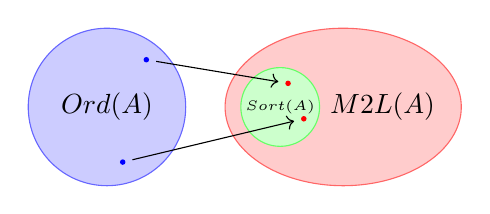
\begin{tikzpicture}
        % draw the sets
        \filldraw[fill=blue!20, draw=blue!60] (-1.5,0) circle (1cm);
        \filldraw[fill=red!20, draw=red!60] (1.5,0) ellipse (1.5cm and 1cm);
        \filldraw[fill=green!20, draw=green!60] (0.7,0) circle (0.5cm);
    
        % the texts
        \node at (-1.5,0) {$\Ord(A)$};
        \node at (0.7, 0) {\tiny$\Sort(A)$};
        \node at (2,0) {$\setmtol(A)$};

    
        % the points in the sets (here I just create nodes to use them later on to position
        % the circles and the arrows
        \node (x1) at (-1,0.6) {};
        \node (x2) at (-1.3,-0.7) {};
        \node (y1) at (0.8,0.3) {};
        \node (y2) at (1,-0.15) {};
    
        % position the elements in the sets (at the nodes we just created)
        \fill[blue] (x1) circle (1pt);
        \fill[blue] (x2) circle (1pt);
        \fill[red] (y1) circle (1pt);
        \fill[red] (y2) circle (1pt);
    
        % draw the arrows
        \draw[->] (x1) -- (y1);
        \draw[->] (x2) -- (y2);
    \end{tikzpicture}
\end{center}

\begin{itemize}
    \item $\Ord(A)$ is the set of \alert{total orders} on $A$,
    \item $\Sort(A)$ is the set of \alert{sorting functions} on $A$,
    \item $\setmtol(A)$ is the set of functions $\term{UnorderedList}(A) \to \List(A)$.
\end{itemize}

Free monoids are lists, free commutative monoids are \alert{unordered lists}!

What properties does $f \in \Sort(A)$ satisfy?

\end{frame}

\begin{frame}{\inline{List} vs \inline{SList}}
Let $\LL(A)$ be the \alert{free monoid}, and $\MM(A)$ the \alert{free commutative monoid} on $A$.

\adjustbox{scale=1.3,center}{%
% https://q.uiver.app/#q=WzAsMixbMCwwLCJcXExMKEEpIl0sWzMsMCwiXFxNTShBKSJdLFsxLDAsInMiLDAseyJjdXJ2ZSI6LTF9XSxbMCwxLCJxIiwwLHsiY3VydmUiOi0xfV1d
\begin{tikzcd}[ampersand replacement=\&,cramped]
	{\LL(A)} \&\&\& {\MM(A)}
	\arrow["s", curve={height=-6pt}, from=1-4, to=1-1]
	\arrow["q", curve={height=-6pt}, two heads, from=1-1, to=1-4]
\end{tikzcd}
}

$q$ is the \alert{canonical map} (surjection) from $\LL(A)$ to $\MM(A)$ (given by extending ${\eta_A^{\MM}}$).

Axiom of Choice says every surjection has a section!

\begin{qblock}
    Constructively, does $q$ have a section?
\end{qblock}

To give a section is to turn an \alert{unordered list} into an \alert{ordered list}.
How should $s$ order the elements? By sorting! (which requires a \alert{total order} on $A$\ldots)

We will show that sorting can be axiomatized from this point of view.

%% Assume we have a \alert{section} $s$ to $q$, that is, for all $x$, $q(s(x)) = x$.

%% We write $[x,y,z]$ for ordered lists, $\{x,y,z\}$ for unordered lists.

%% But, there are many sections. A correct sorting algorithm is a well-behaved section.

%% $s$ picks a canonical representation out of the equivalence classes generated by commutativity,
%% is it doing sorting?
    
\end{frame}

\begin{frame}{Sorting}
Informally, we prove:
\begin{enumerate}
    \item if A has a decidable total order, there is a well-behaved section.
    \item if there is a well-behaved section, A is totally ordered.
\end{enumerate}

This \alert{well-behaved section} gives a \alert{correct sort function}!

Axioms of \alert{total order}:
\begin{itemize}
    \item reflexivity: $x \leq x$
    \item transitivity: if $x \leq y$ and $y \leq z$, then $x \leq z$
    \item antisymmetry: if $x \leq y$ and $y \leq x$, then $x = y$
    \item totality: forall $x$ and $y$, we have \alert{merely} either $x \leq y$ or $y \leq x$ 
\end{itemize}

\begin{pblock}
    Assume there is a decidable total order on $A$.
    There is a sort function $s\colon \MM(A) \to \LL(A)$ which constructs a section to $q\colon \LL(A) \twoheadrightarrow \MM(A)$.
\end{pblock}

We can construct a section $s$ by any sorting algorithm, we chose \alert{insertion sort}.

\end{frame}


\begin{frame}{Sorting}

To go the other way, given a section $s$, 
we can construct a relation that satisfies \alert{reflexivity}, \alert{antisymmetry}, and \alert{totality}!

\begin{dblock}
    Given a section $s$, define:
    \begin{align*}
        \text{least}(xs) & \coloneqq \text{head}(s(xs)) \\
        x \preceq y      & \coloneqq \text{least}(\{x, y\}) \id x
    \end{align*}
\end{dblock}

We prove:
\begin{itemize}
    \item \alert{reflexivity}: $x \preceq x$:
    
    $\text{least}(\{x, x\}))$ must be x.
    
    \item \alert{antisymmetry}: if $x \preceq y$ and $y \preceq x$, then $x = y$:
    
    $x = \text{least}(\{x, y\}) = y$
    
    \item \alert{totality}: for all $x$ and $y$, either $x \preceq y$ or $y \preceq x$:
    
    $\text{least}(\{x, y\})$ is merely either $x$ or $y$.
    
\end{itemize}

But what about \alert{transitivity}?

\end{frame}

\begin{frame}{Sorting}

%% But what about \alert{transitivity}?

Consider this section $s : SList(\Nat) \to List(\Nat)$:

\begin{align*}
    s(xs) & = \begin{cases}
        \text{sort}(xs)                  & \text{if length($xs$) is odd}   \\
        \text{reverse}(\text{sort}(xs))  & \text{otherwise}
    \end{cases} \\
    s(\{2,3,1,4\}) & = [4,3,2,1] \\
    s(\{2,3,1\}) & = [1, 2, 3]
\end{align*}

$s$ doesn't sort and violates \alert{transitivity}!

A correct sort function needs more constraints \ldots
    
\end{frame}

\begin{frame}{Correctness of Sorting}

%% But what about \alert{transitivity}?
%% More constraint is needed...
Given a section $s$:

\begin{dblock}[is-sorted]
    A list $xs$ is sorted if $\exists ys. \, s(ys) = xs$.
\end{dblock}

\begin{dblock}[is-head-least]
    $s$ satisfies \textit{is-head-least} if \\
    $\forall x \, xs. \, \text{is-sorted}(x :: xs) \land y \in (x :: xs) \to \text{is-sorted}([x, y])$.
\end{dblock}

\begin{tblock}[Lemma]
    \alert{\textit{is-head-least}} is equivalent to \alert{transitivity} of $\preceq$.
\end{tblock}

\begin{tblock}[Corollary]
    If $s$ satisfies {\textit{is-head-list}}, then $\preceq$ is a total order on $A$.
\end{tblock}

\end{frame}

\begin{frame}{Axiomatics of Sorting}

    Next step: we want to upgrade this proof to an equivalence between total orders on $A$, and well-behaved sections $s$.

    Given a \alert{decidable total order} $\leq$, we use it to construct a sort function (e.g. insertion sort).
    Insertion sort satisfies \textit{is-head-least}, and we use it to construct a total order $\preceq$.

    \begin{pblock}[Question]
        \begin{itemize}
            \item Is $\preceq \, = \, \leq$?
            \item If we use $s$ to construct $\preceq$, can we reconstruct $s$ from $\preceq$?
        \end{itemize}        
    \end{pblock}

    As it turns out, \textit{is-head-least} is \alert{not enough} to axiomatize sorting functions!
\end{frame}

\begin{frame}{Axiomatics of Sorting}

If we use $s$ to construct $\preceq$, can we reconstruct $s$ from $\preceq$? 

Let sort be insertion sort by $\preceq$. Consider this section $s : SList(\Nat) \to List(\Nat)$:

\begin{align*}
    s(xs) & = \text{least}(xs) :: \text{reverse(tail(sort($xs$)))} \\
    s(\{2,3,1,4\}) & = [1,4,3,2] \\
    s(\{2,3,1\}) & = [1, 3, 2]
\end{align*}

$s$ is not the same as insertion sort, but both give us the same $\preceq$!

We need another constraint: %% to get a \alert{full equivalence}:

\begin{dblock}[is-tail-sort]
    A section $s$ satisfies \textit{is-tail-sort} if: \\
    $\forall x \, xs. \, \text{is-sorted}(x :: xs) \to \text{is-sorted}(xs)$.
\end{dblock}
    
\end{frame}


\begin{frame}{Main Result}
Our final theorem:
\begin{dblock}
    \begin{itemize}
        \item $\type{DecTotOrd}(A)$ = decidable total orders on $A$

        \item $\type{Sort}(A)$ = sections $s\colon \MM(A) \to \LL(A)$ to $q$,
            satisfying $\term{is-head-least}$ and $\term{is-tail-sort}$,
            where $A$ has decidable equality
    \end{itemize}
\end{dblock}

\begin{tblock}
    $\term{o2s}\colon \type{DecTotOrd}(A) \to \type{Sort}(A)$ is an equivalence.
\end{tblock}

There is a \alert{decidable total order} on $A$ iff
$A$ has \alert{decidable equality} and a \alert{section} satisfying $\term{is-head-least}$ and $\term{is-tail-sort}$!

\end{frame}
\begin{frame}{Main Result}

\begin{tblock}
    $\term{o2s}\colon \type{DecTotOrd}(A) \to \type{Sort}(A)$ is an equivalence.
\end{tblock}

Given $\type{DecTotOrd}(A)$:
\begin{itemize}
    \item We can construct a section $s\colon \MM(A) \to \LL(A)$ with \alert{insertion sort},
    which satisfies $\term{is-head-least}$ and $\term{is-tail-sort}$
    \item We can show $A$ has \alert{decidable equality} by determining if $x \leq y$ and $y \leq x$,
    antisymmetry gives us $x = y$ if $x \leq y$ and $y \leq x$
\end{itemize}

Given $\type{Sort}(A)$:
\begin{itemize}
    \item We can construct a \alert{total order} $x \, \preceq \, y := least(\{x, y\}) = x$ as shown previously
    \item Because A has decidable equality, we can determine $least(\{x, y\}) = x$, so $\preceq$ is \alert{decidable}
\end{itemize}

\end{frame}

\begin{frame}{Main Result}

\begin{tblock}
    $\term{o2s}\colon \type{DecTotOrd}(A) \to \type{Sort}(A)$ is an equivalence.
\end{tblock}

It's an equivalence!
\begin{itemize}
    \item $\type{DecTotOrd}(A) \xto{o2s} \type{Sort}(A) \xto{o2s^{-1}} \type{DecTotOrd}(A)$
    \begin{itemize}
        \item $\text{least}(\{x, y\}) = x \text{ iff } x \leq y$
    \end{itemize}

    \item $\type{Sort}(A) \xto{o2s^{-1}} \type{DecTotOrd}(A) \xto{o2s} \type{Sort}(A)$
    \begin{itemize}
        \item Given a section $s$ that satisfies \alert{is-head-least} and \alert{is-tail-sort},
              $s$ is equal to insertion sort with the order $\preceq$ generated by $s$.
        \item \alert{is-head-least} lets us create the \alert{total order} $\preceq$.
        \item \alert{is-tail-sort} lets us inductively prove that $s$ \alert{sorts} the list by $\preceq$.
        \item Both $s$ and insertion sort produce lists sorted by $\preceq$, and they're the same!
    \end{itemize}
\end{itemize}

\end{frame}


\begin{frame}{Main Result}

  \begin{qblock}
    What is a correct sorting algorithm?
  \end{qblock}

  \begin{pblock}[Answer]
  A sort function is a section $s\colon \MM(A) \to \LL(A)$ to the canonical map $q\colon \LL(A) \twoheadrightarrow \MM(A)$,
  satisfying:
  \begin{itemize}
      \item \textit{is-head-least}: $\forall x \, xs. \, \text{is-sorted}(x :: xs) \land y \in (x :: xs) \to \text{is-sorted}([x, y])$,
      \item \textit{is-tail-sort}: $\forall x \, xs. \, \text{is-sorted}(x :: xs) \to \text{is-sorted}(xs)$.
  \end{itemize}
  where $xs$ \textit{is-sorted} if it is in the truncated fiber of $s$.
  \end{pblock}

  \begin{tblock}[Remarks]
  \begin{itemize}
      \item Other specifications of sorting (in Coq, or the VFA livre) are given in terms of \inline{sort : List Nat -> List Nat}.
      \item These are special cases of our axiomatic understanding of sorting!
  \end{itemize}
  \end{tblock}
\end{frame}

\begin{frame}{Future work}

\begin{itemize}
  \item How does this observation relate to the Axiom of Choice?
    \begin{itemize}
      \item Axiom of Choice is equivalent to the Well-ordering principle. %%: ``every set is well-ordered''.
        \item We have shown this is equivalent to having a correct sort function.
        \item Study the connections with constructive taboos in HoTT.
    \end{itemize}
    \item Sorting is not just about extensional correctness:
    \begin{itemize}
        \item How do different sorting algorithms fit into this picture?
        \item Related:~\cite{hinzeSortingBialgebrasDistributive2012}.
    \end{itemize}    
    \item From sets to groupoids:
    \begin{itemize}
        \item Is any symmetric monoidal groupoid symmetric monoidal equivalent to a commutative monoidal groupoid?
    \end{itemize}
    \item Framework for universal algebra:
    \begin{itemize}
        \item Constructions of free objects for varieties of algebras.
        \item Categorify from sets to groupoids, going from system of equations to system of coherences.
    \end{itemize}
\end{itemize}

\end{frame}

\begin{frame}[standout]
    Thank you!
\end{frame}

% \nocite{*}

\begin{frame}[allowframebreaks]
    \frametitle{References}
    \printbibliography[heading=none]
\end{frame}

\end{document}
